\documentclass{standalone}
\usepackage{tikz}

\begin{document}

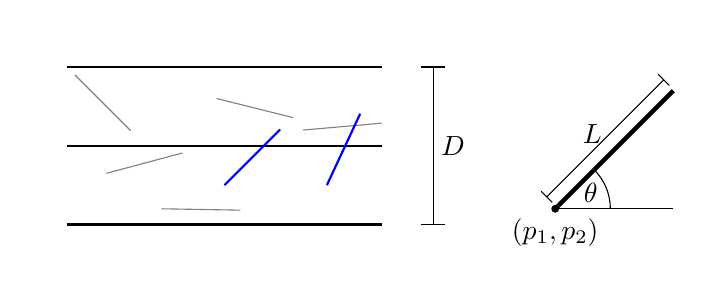
\begin{tikzpicture}
    \fill[white] (-6.5,1.5) rectangle (2,-1.5);
    \draw [thick] (-6, 1) -- (-2, 1);
    \draw [thick] (-6, 0) -- (-2, 0);
    \draw [thick] (-6,-1) -- (-2,-1);
    
    % dropped needles
    \draw [gray] (-5.5, -0.35) -- ++(15:1cm);
    \draw [gray] (-5.9, 0.9) -- ++(-45:1cm);
    \draw [gray] (-3, 0.2) -- ++(5:1cm);
    \draw [gray] (-4.1, 0.6) -- ++(-14:1cm);
    \draw [gray] (-4.8, -0.8) -- ++(-1:1cm);

    % dropped needles, cross line
    \draw [thick, blue] (-2.7, -0.5) -- ++(65:1cm);
    \draw [thick, blue] (-4, -0.5) -- ++(45:1cm);

    \draw (-1.2, 1) -- (-1.5, 1);
    \draw (-1.35, 1) -- (-1.35, -1);
    \draw (-1.2, -1) -- (-1.5, -1);
    \node (foo) at (-1.1, 0) {$D$};

    % \draw (-0.2, 1.2) -- (-0.2, -1.2) -- (2, -1.2);
    \fill (0.2, -0.8) circle (0.05);
    \node[anchor=north] (foo) at (0.2, -0.8) {$(p_1,p_2)$};
    \draw[ultra thick] (0.2, -0.8) -- (1.7, 0.7);
    \draw (1.7, -0.8) -- (0.2, -0.8);
    \draw (0.9, -0.8) arc (0:45:0.7cm);
    \node (foo) at (0.65, -0.6) {$\theta$};
    \begin{scope}[shift={(0.87 cm,0.13 cm)},rotate=45]
        \node (foo) at (-0.13, 0.15) {$L$};
        \draw (-1.1, 0.1) -- (-1.1, -0.1);
        \draw (1, 0.1) -- (1, -0.1);
        \draw (-1.1, 0) -- (1, 0);
    \end{scope}
\end{tikzpicture}

\end{document}